%% eval.tex
%% $Id: eval.tex 61 2012-05-03 13:58:03Z bless $

\chapter{Evaluation}
\label{ch:Evaluation}
%% ==============================

We are free to choose what states are substituted and used in the decomposition algorithm and further on, either the ones or the zeros from the label. Intuitively, there are less ones than zeroes in the original data, therefore less periods need to be found and less values to be mapped, which in turn should increase speed and effectiveness, therefore initially ones were substituted. For the empirical analysis of the decomposition, each edge of each graph of the collection is decomposed into periods and then the periods are collected until they align to give the original data. All the periods are evaluated and also visualized directly in code with the help of Lets-Plot\footnote{\url{https://lets-plot.org/}}.

\begin{figure}[!htb]
	\centering
	\begin{minipage}{.5\textwidth}
		\centering
		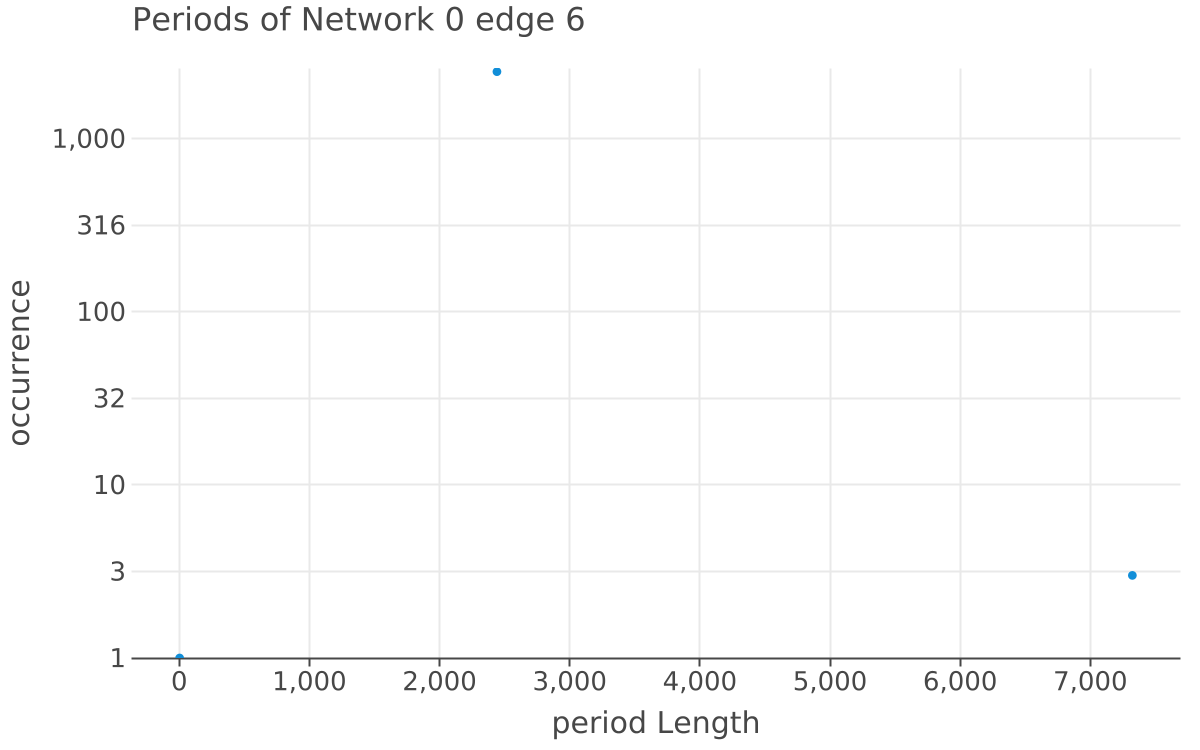
\includegraphics[width=\linewidth]{charts/introduction/test-edge-plot-log.png}
		\\ A subfigure
		\label{fig:intro-edge-plot}
	\end{minipage}%
	\begin{minipage}{0.5\textwidth}
		\centering
		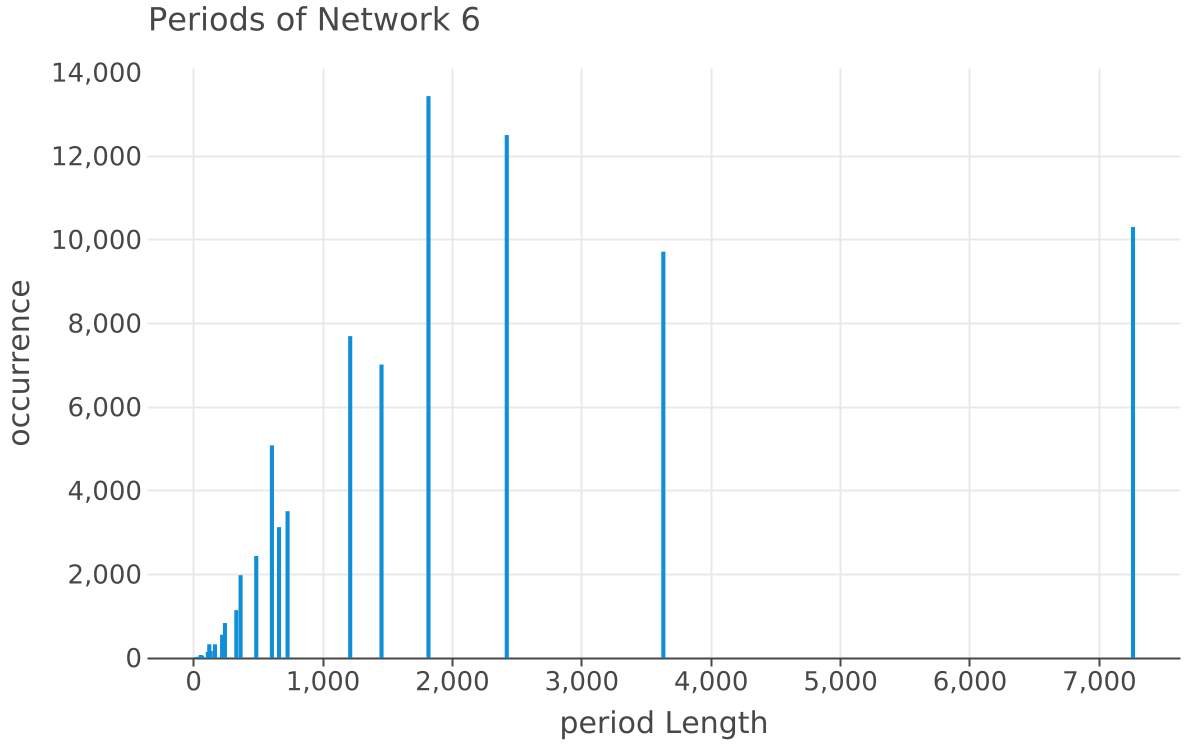
\includegraphics[width=\linewidth]{charts/introduction/test-graph-plot.png}
		\\ A subfigure
		\label{fig:intro-graph-plot}
	\end{minipage}
\end{figure}

When looking at a single edge of a single graph (edge 6 of network 0 in this case), the picture is clear. We find one very short period of length 3, around 2k periods of length 2441 ($\frac{1}{3}$ of the original size) and 3 outliers with original length of 7323. If we collect and analyze the periods for all edges of a single graph, it looks somewhat similar, a couple small and some of $\frac{1}{3}$ or $\frac{1}{4}$ the original size and then all remaining outliers.  This gives some insight into the resulting composition of periods depending on the parameters and can be done for the whole set of real world data. Besides the total amount of periods of different length, it is also interesting to see how many values are covered by what type of period, which will be done later in this section.

\begin{figure}[h]
	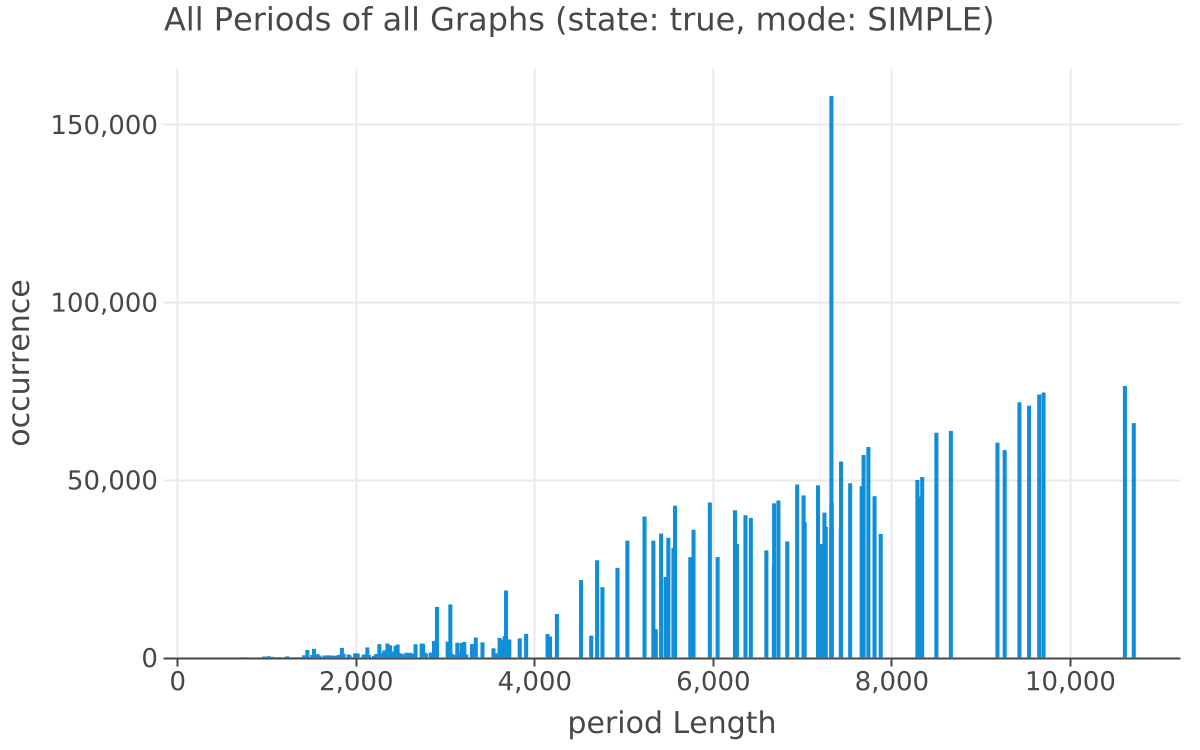
\includegraphics[width=\linewidth]{charts/all-graphs-bar-char-strue-mSIMPLE.png}
	\caption{TODO}
	\label{fig:plot-all-periods-true-state}
\end{figure}

\section{Empirical analysis of the decomposition}

In total, 3.1 mil values have been covered with a total of 2.8 mil periods, so on average a single period only covered 1.095 values from the input label. This is also visible in the bar chart in figure \ref{fig:plot-all-periods-true-state}, where there are some smaller periods present with a period length around 2000 but the main bulk has a period length larger than 4000. Switching the state to substitute to false, increases the amount of states to represent but also the chances of finding shorter periods which cover more than one value on average.

\begin{figure}[h!]
	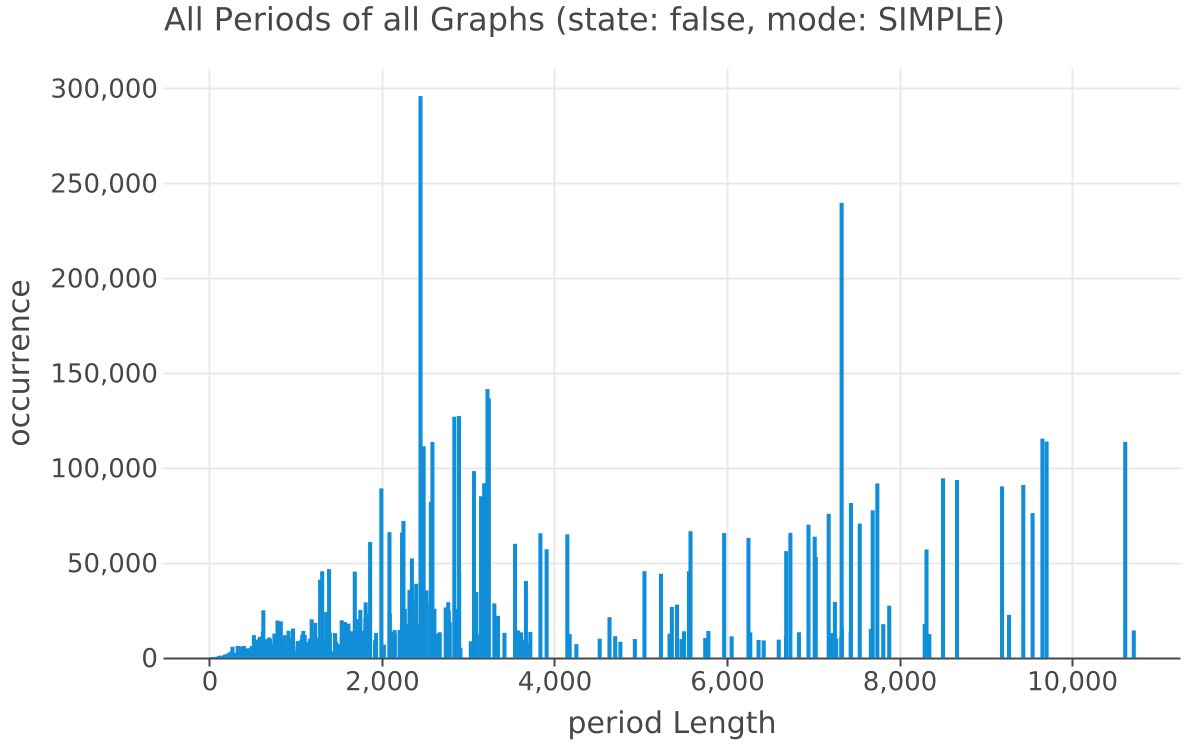
\includegraphics[width=\linewidth]{charts/all-graphs-bar-char-sfalse-mSIMPLE.png}
	\caption{TODO}
	\label{fig:plot-all-periods-false-state}
\end{figure}

Looking at the evaluation of substituting zeroes in figure \ref{fig:plot-all-periods-false-state}, a mixed image is visible. The amount of values to cover as well as the amount of periods increased to 20 mil values and a total of 7.3 mil periods. This means an improvement to 2.73 values per period on average but also a 7x increased amount of periods.


\section{Values covered by type of period}

\begin{figure}[h!]
	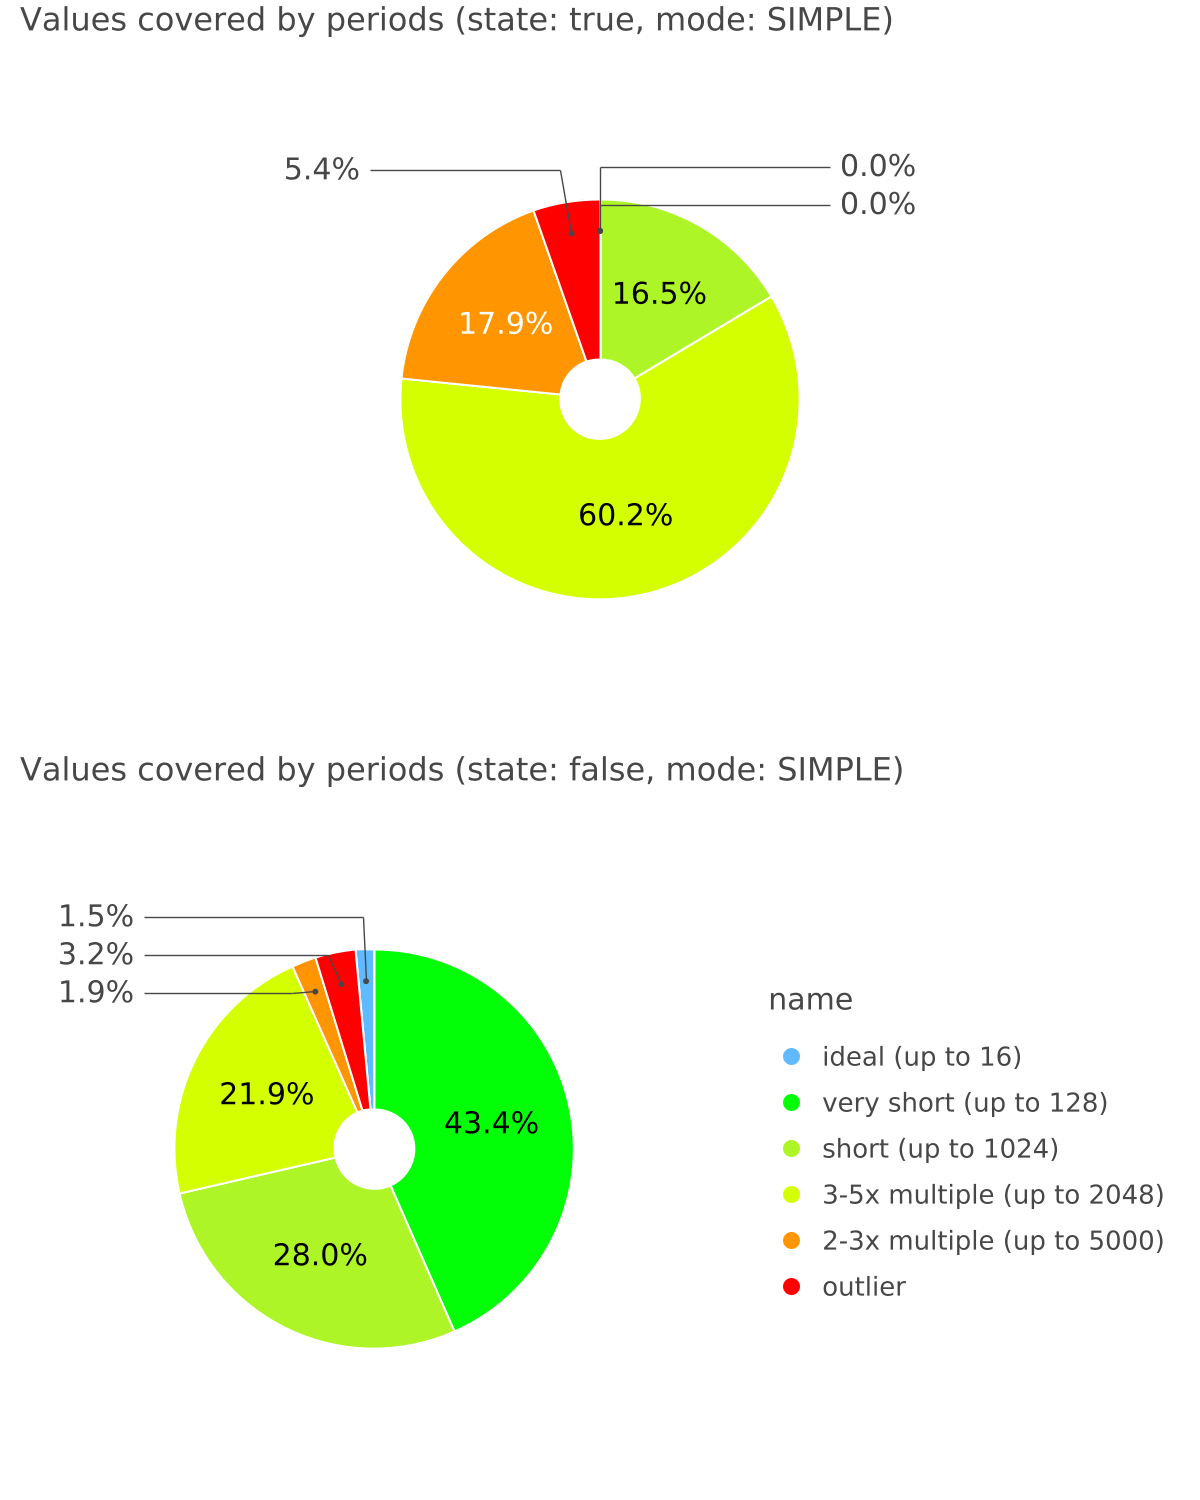
\includegraphics[width=\linewidth]{charts/all-covered-values-pie-chart-combined-ontop.png}
	\caption{A subfigure}
	\label{fig:plot}
\end{figure}

%%% Local Variables: 
%%% mode: latex
%%% TeX-master: "thesis"
%%% End: 
